\documentclass[conference]{IEEEtran}

% Encodage/typo
\usepackage[T1]{fontenc}
\usepackage[utf8]{inputenc}
\usepackage[english]{babel}
\usepackage{microtype}

% Math
\usepackage{amsmath, amssymb}

% Figures
\usepackage{graphicx}
\DeclareGraphicsExtensions{.pdf,.png,.jpg}
\graphicspath{{images/}}

% Subfigures compatibles IEEE (éviter subcaption)
\usepackage[caption=false,font=footnotesize]{subfig}

% à AJOUTER pour forcer l'écoulement des figures par section/bloc
\usepackage[section]{placeins} 

% Floats pleine largeur en haut/bas (figure* / table*)
\usepackage{stfloats}

% Tables
\usepackage{booktabs}

% Liens
\usepackage{hyperref}


\title{Anomaly Detection in Microservice-based Applications:
A Comparative Study of Machine Learning Models}

\author{
\IEEEauthorblockN{Darius TEMGOUA}
\IEEEauthorblockA{\textit{Université de Yaoundé I} \\
Yaoundé, Cameroun \\
steves.temgoua@facsciences-uy1.cm}
\and
\IEEEauthorblockN{Valéry MONTHE}
\IEEEauthorblockA{\textit{Université de Yaoundé I} \\
Yaoundé, Cameroun \\
valery.monthe@facsciences-uy1.cm}
}


\begin{document}

\maketitle

\begin{abstract}
In a constantly evolving landscape where modern software systems are increasingly adopting distributed architectures, microservices are emerging as a crucial solution. However, their distributed nature and high interconnectivity make monitoring and anomaly detection particularly challenging, as traditional methods do not always provide effective resilience. This thesis proposes a comparative study of different machine learning approaches applied to anomaly detection in microservice-based systems.
The objective is to highlight the real capabilities of models such as the multi-layer perceptron (MLP), the LSTM autoencoder, and a hybrid model combining sequential representation and supervised classification.

The experimental study is based on a dataset in which anomaly data were injected to simulate the behavior of applications at the service level and the global application level. After rigorous data preprocessing, the models were trained and then evaluated according to classic metrics (accuracy, precision, recall, F1-score) and the results reveal that despite the complexity of some models, the overall performances remain close, suggesting that in a low-noise and low-dimensional environment, simple models can be sufficient to detect anomalies effectively.

This study is part of a DevOps context in order to propose monitoring tools capable of contributing to the resilience of distributed systems.
\end{abstract}

\renewcommand{\IEEEkeywordsname}{Keywords}
\begin{IEEEkeywords}
DevOps, Distributed monitoring, Microservices, Anomaly detection, Machine learning, Comparative study.
\end{IEEEkeywords}


\section{Introduction}
L’essor des architectures microservices, désormais standard dans le développement d’applications distribuées, offre modularité, résilience et flexibilité, mais complexifie considérablement la surveillance. Chaque service produit ses propres métriques, journaux et traces, rendant difficile la détection précoce d’anomalies, surtout dans des environnements DevOps à cycles de déploiement rapides en l'occurence avec les outils CI/CD. Les approches traditionnelles, basées sur des seuils ou règles statiques, peinent à capter les dynamiques séquentielles des données et manquent de flexibilité face à l’évolution constante des systèmes.

La détection proactive d’anomalies revêt une importance stratégique : elle limite les interruptions de service, réduit les pertes financières, renforce la satisfaction client et garantit la continuité d’activité, particulièrement dans des secteurs critiques comme les télécommunications ou la santé. Dans un contexte DevOps, elle permet de diminuer significativement le \cite{Morais2023_mttd_mttr} \textbf{Mean Time to Detect (MTTD)} et le \textbf{Mean Time to Repair (MTTR)}, améliorant à la fois la productivité et la qualité de service.

Face à ces enjeux, l’apprentissage automatique (\textbf{machine learning}) s’impose comme une piste prometteuse. Ce travail explore une question centrale : \textbf{\textit{dans quelle mesure la complexité d’un modèle améliore-t-elle la détection d’anomalies dans un environnement microservices ?}} En particulier, \textit{les modèles avancés comme les autoencodeurs LSTM offrent-ils un avantage tangible par rapport à des approches plus simples telles que les perceptrons multicouches ?}

L’objectif ici est de proposer une solution pratique et reproductible de détection d’anomalies adaptée aux environnements microservices, en comparant les performances de modèles de complexité variable à partir de données simulées réalistes, et en analysant l’impact de cette complexité sur la qualité de détection.

% ===========================
% RELATED WORKS
% ===========================
\section{Related Works}
La détection d’anomalies dans les systèmes microservices est un domaine de recherche actif, ceci en raison de la complexité croissante des architectures distribuées et de la nécessité d’assurer leur résilience.
Plusieurs travaux de recherche récents ont proposé des approches innovantes pour traiter les défis associés à l'oservabilité et à l'analyse des performances de ces systèmes, en s’appuyant sur différents types de données et techniques d’apprentissage automatique.

\begin{itemize}
\item Behera et al. \cite{behera2023_model_of_anomalie} (2023) ont proposé une approche comparative pour la détection d'anomalies dans les journaux de log non structurés générés par des microservices, en utilisant trois méthodes non supervisées : \textbf{Isolation Forest (IF)}, \textbf{One-Class SVM (OC-SVM)} et \textbf{Local Outlier Factor (LOF)}. Les résultats expérimentaux montrent des précisions élevées (98\%-99\%) avec IF et LOF générant moins de faux positifs que OC-SVM, tandis que ce dernier se distingue par une sensibilité accrue aux anomalies isolées.
\item Grambow et al. \cite{grambow2020} (2020) proposent une approche basée sur des modèles d'interaction abstraits pour le benchmarking des microservices, soulignant l'importance de la représentation des interactions au sein des systèmes distribués. Cependant, peu d'études exploitent les traces pour la détection d'anomalies de manière efficace. Certaines approches, comme celles de Wang et al. (2019), se concentrent sur la comparaison de traces pour détecter des anomalies, mais peuvent s'avérer coûteuses en termes de calcul et moins adaptées à des scénarios en temps réel.

\item Bogatinovski et al. \cite{bogatinovski2020} (2020) ont proposé une méthode d’apprentissage auto-supervisée basée sur les traces distribuées. Leur approche encode les séquences d’appels de services pour construire une représentation latente, utilisée ensuite pour identifier les anomalies sans supervision explicite.

\item Nobre et al. \cite{nobre2023} (2023) ont réalisé une étude approfondie sur les défis de la détection d’anomalies dans les architectures microservices. Leur travail met en avant l’efficacité du Perceptron Multi-Couche (MLP) pour la détection au niveau service, en montrant des scores F1 élevés sur des jeux de données injectés de fautes. Ils insistent sur la nécessité de disposer de jeux de données réalistes pour mieux entraîner les modèles.

\item Silva et al. \cite{silva2022_auto_encodeur} (2022) ont développé un système de détection d’anomalies en exploitant des autoencodeurs dans un environnement Kubernetes. En utilisant des outils comme eBPF pour collecter des métriques noyau fines, ils ont montré que les autoencodeurs peuvent détecter efficacement les anomalies dans des contextes dynamiques à forte volumétrie.

\item Raeiszadeh et al. \cite{Raeiszadeh2023} (2023) ont introduit une approche de détection en temps réel des anomalies à partir des traces distribuées dans les systèmes cloud à base de microservices. Leur modèle repose sur l’encodage des séquences de services et l’analyse en ligne des écarts de comportement, avec une attention particulière portée à la latence de détection.

\end{itemize}

Chacune de ces approches souligne l’importance d’adapter la méthode de détection aux types de données disponibles (logs, métriques, traces), aux contraintes du système (temps réel, volumétrie, distribution) et aux objectifs visés (performance, sécurité, fiabilité).

\section{Methodology}
\subsection{Dataset Description}

Les expérimentations de ce travail s'appuient sur un jeu de données proposé par \cite{nobre2023}, spécialement conçu pour l’étude de la détection d’anomalies dans des environnements microservices. Ce jeu de données présente l’avantage d’être \textbf{scientifiquement contrôlé} et \textbf{reproductible}, ce qui le rend particulièrement adapté à la comparaison objective de modèles d’apprentissage automatique.

\subsubsection{Structure et granularité}
Le jeu de données est structuré selon deux niveaux d’analyse.
\begin{itemize}
    \item \textbf{Niveau service} : chaque observation correspond aux mesures d’un service individuel à un instant donné. Les principales variables incluent :
    \begin{itemize}
        \item \texttt{Mean} : temps de réponse moyen (en ms) ;
        \item \texttt{50th quantile} : médiane des temps de réponse, reflétant la performance typique ;
        \item \texttt{99th quantile} : temps de réponse du pire cas observé ;
        \item \texttt{2xx} : nombre de requêtes HTTP réussies ;
        \item \texttt{4xx} / \texttt{5xx} : nombre de réponses HTTP erronées côté client ou serveur.
    \end{itemize}
    \item \textbf{Niveau application} : données agrégées provenant de plusieurs services, offrant une vision globale du comportement du système.
\end{itemize}

\subsubsection{Processus de génération et de collecte}
L’environnement de collecte mis en place par \cite{nobre2023} comprend.
\begin{itemize}
    \item un \textbf{cluster Kubernetes} hébergeant un ensemble de microservices simulant une application complète ;
    \item un outil de monitoring (\textit{Prometheus}) collectant les métriques toutes les 15 secondes ;
    \item un \textbf{mécanisme d’injection d’anomalies} permettant de simuler différents scénarios :
    \begin{itemize}
        \item augmentation artificielle de la latence ;
        \item génération d’erreurs HTTP (4xx et 5xx) ;
        \item arrêt ou indisponibilité de services.
    \end{itemize}
\end{itemize}

Les anomalies sont injectées de manière isolée ou combinée, reproduisant des situations réalistes tout en conservant une maîtrise expérimentale.

\subsubsection{Étiquetage des données}
Chaque observation est associée à une variable binaire \texttt{IsError} définissant l’état du système :
\[
y =
\begin{cases}
0, & \text{comportement normal} \\
1, & \text{comportement anormal}
\end{cases}
\]
Les données se présentent ainsi sous la forme :
\[
X \in \mathbb{R}^{n \times p}, \quad y \in \{0,1\}^n
\]
où $n$ est le nombre d’observations et $p$ le nombre de variables.

\subsection{Preprocessing}

Le prétraitement des données est une étape déterminante, car la qualité de cette phase conditionne directement les performances et la stabilité des modèles d’apprentissage automatique.  
Les opérations suivantes ont été effectuées pour garantir des entrées propres, homogènes et exploitables.

\subsubsection{Nettoyage et préparation}
\begin{itemize}
    \item \textbf{Conversion des timestamps} : transformation des horodatages en format temporel exploitable pour l’indexation et la synchronisation des données ;
    \item \textbf{Harmonisation des types de données} : conversion explicite des colonnes numériques et catégorielles dans des formats appropriés ;
\end{itemize}

\subsubsection{Normalisation des variables}
Les variables présentant des échelles différentes (par exemple, temps en millisecondes et taux d’erreurs en pourcentage) ont été ramenées sur une échelle commune via un \textit{Min-Max Scaling} :
\[
x_{\text{scaled}} = \frac{x - \min(x)}{\max(x) - \min(x)}
\]
Cette transformation garantit que toutes les variables contribuent de manière équilibrée à l’apprentissage, en évitant qu’une seule domine le processus.

\subsection{Models Evaluated}

Afin de couvrir différentes approches d’apprent issage, trois modèles ont été retenus dans le cadre de cette étude :  
\begin{enumerate}
    \item un modèle supervisé classique pour données tabulaires ;
    \item un modèle non supervisé adapté aux séries temporelles ;
    \item un modèle hybride combinant deux paradigmes.
\end{enumerate}

\subsubsection{Perceptron Multicouche (MLP)}
Le Perceptron Multicouche (\textit{Multi-Layer Perceptron}, MLP) a été implémenté à l’aide de la bibliothèque \texttt{scikit-learn}.  
Ce réseau de neurones \textit{feedforward}~(l'information circule des neurones d'entrés vers les neurones de sortie, sans aucun retour ou boucle) est structuré comme suit :
\begin{itemize}
    \item \textbf{Couche d’entrée} : reçoit les variables explicatives prétraitées ;
    \item \textbf{Couches cachées} : entre 4 et 16 neurones avec des fonctions d’activation non linéaires telles que \texttt{ReLU} ou \texttt{tanh} ;
    \item \textbf{Couche de sortie} : un seul neurone activé par une fonction \texttt{sigmoïde}, produisant une probabilité d’appartenance à la classe \texttt{anomalie}.
\end{itemize}
L’optimisation a été réalisée avec les solveurs \texttt{adam} (rapide et adaptatif) et \texttt{lbfgs} (plus stable pour petits ensembles de données).  
Une recherche d’hyperparamètres (\texttt{GridSearchCV}) a été menée pour ajuster la profondeur, le taux d’apprentissage et la régularisation.  

\subsubsection{Autoencodeur LSTM}
L’Autoencodeur LSTM (\textit{Long Short-Term Memory Autoencoder}) a été développé avec \texttt{Keras/TensorFlow} afin d’exploiter les dépendances temporelles présentes dans les données des microservices.
Ce modèle, de nature non supervisée, fonctionne en trois étapes :
\begin{enumerate}
    \item \textbf{Encodage} : une ou plusieurs couches LSTM (16 à 32 unités) compressent la séquence d’entrée dans une représentation latente compacte ;
    \item \textbf{Décodage} : reconstruction de la séquence initiale à partir de cette représentation ;
    \item \textbf{Évaluation} : l’erreur de reconstruction est utilisée comme score d’anomalie, et un seuil empirique (déterminé sur un ensemble de validation) permet de classer l’observation.
\end{enumerate}
Les fonctions d’activation \texttt{tanh} et la perte \texttt{MSE} (\textit{Mean Squared Error}) ont été utilisées.  
L’entraînement s’est déroulé uniquement sur des séquences normales, sur 10 à 15 époques, avec une taille de lot (\textit{batch size}) de 16 et l’optimiseur \texttt{Adam}. \textit{EarlyStopping} à été utilisé pour éviter le surapprentissage en surveillant la \texttt{validation loss}.

\subsubsection{Modèle Hybride MLP + LSTM}
Le modèle hybride combine deux sous-architectures :
\begin{itemize}
    \item une \textbf{branche LSTM} dédiée à l’analyse des variables séquentielles (métriques temporelles collectées dans le temps) ;
    \item une \textbf{branche dense (MLP)} pour traiter les variables statiques ou dérivées ne possédant pas de structure temporelle.
\end{itemize}
Les sorties de ces deux branches sont concaténées, puis transmises à une couche dense finale avec activation \texttt{sigmoïde}.
L’entraînement est réalisé sur 10 à 15 époques, avec un \texttt{dropout} compris entre 0,2 et 0,5 pour limiter le surapprentissage.
Ce type d’architecture permet de capturer simultanément :
\begin{itemize}
    \item les \textbf{dynamiques temporelles} via la branche LSTM ;
    \item les \textbf{relations instantanées} via la branche dense.
\end{itemize}
Cette combinaison est particulièrement pertinente dans le contexte microservices, où certaines anomalies se manifestent par des ruptures dans les tendances temporelles tandis que d’autres sont visibles à un instant donné.

\subsection{Experimental Setup}

Cette section décrit l’environnement logiciel et matériel utilisé pour les expérimentations, ainsi que les métriques et outils d’évaluation mobilisés.

\subsubsection{Environnement logiciel}
Les expérimentations ont été menées en \textbf{Python 3.x}, avec les bibliothèques suivantes :
\begin{itemize}
    \item \texttt{Pandas}, \texttt{NumPy} : manipulation et structuration des données ;
    \item \texttt{Matplotlib}, \texttt{Seaborn} : visualisation et analyse graphique ;
    \item \texttt{Scikit-learn} : implémentation du MLP, prétraitement des données et calcul des métriques d’évaluation ;
    \item \texttt{TensorFlow/Keras} : implémentation des modèles LSTM Autoencodeur et Hybride.
\end{itemize}

\subsubsection{Configuration matérielle}
Les tests ont été exécutés sur une machine disposant de la configuration suivante :
\begin{itemize}
    \item Processeur : Intel Core i7 (10\textsuperscript{e} génération) ;
    \item Mémoire vive : 32 Go RAM ;
    \item Carte graphique : GPU NVIDIA avec 12 Go de mémoire dédiée.
\end{itemize}

\subsubsection{Métriques d’évaluation}

Plusieurs métriques complémentaires ont été utilisées pour évaluer la performance des modèles.  
Elles permettent d’apprécier la capacité des modèles à distinguer correctement les comportements normaux des anomalies, en particulier dans un contexte de classes déséquilibrées.

\begin{itemize}
    \item \textbf{Accuracy} : proportion totale de prédictions correctes sur l’ensemble du jeu de données.
    \[
    \text{Accuracy} = \frac{TP + TN}{TP + TN + FP + FN}
    \]
    où $TP$ (True Positives) représente les anomalies correctement détectées, $TN$ (True Negatives) les observations normales bien classées, $FP$ (False Positives) les fausses alertes et $FN$ (False Negatives) les anomalies non détectées.
    
    \item \textbf{Precision} : proportion d’anomalies correctement identifiées parmi celles prédites comme telles (réduction des fausses alertes).
    \[
    \text{Precision} = \frac{TP}{TP + FP}
    \]
    
    \item \textbf{Recall (Sensibilité)} : proportion d’anomalies correctement détectées parmi toutes les anomalies présentes (réduction des anomalies manquées).
    \[
    \text{Recall} = \frac{TP}{TP + FN}
    \]
    
    \item \textbf{F1-score} : moyenne harmonique entre la précision et le rappel, offrant un compromis entre les deux.
    \[
    \text{F1-score} = 2 \times \frac{\text{Precision} \times \text{Recall}}{\text{Precision} + \text{Recall}}
    \]
\end{itemize}

Ces métriques sont complétées par des outils visuels pour interpréter les résultats :
\begin{itemize}
    \item \textbf{Matrices de confusion} : représentation de la répartition des vraies et fausses prédictions par classe ;
    \item \textbf{Courbes d’apprentissage} (perte et précision) : suivi de la convergence des modèles au fil des époques ;
    \item \textbf{Distribution des erreurs de reconstruction} : spécifique aux Autoencodeurs LSTM, permettant d’évaluer la séparation entre séquences normales et anormales.
\end{itemize}

Ces éléments assurent une évaluation complète, combinant analyse chiffrée et interprétation visuelle, afin d’identifier les forces et limites de chaque modèle dans le contexte de la détection d’anomalies sur architectures microservices.

% ===========================
% RESULT S AND DISCUSSION
% ===========================
\section{Results and Discussion}

\subsection{Résultats expérimentaux}

Les modèles ont été évalués selon des métriques standards de classification : \textit{accuracy}, \textit{precision}, \textit{recall} et \textit{F1-score}. Les matrices de confusion permettent de visualiser les proportions de vrais positifs (VP), vrais négatifs (VN), faux positifs (FP) et faux négatifs (FN), tandis que les courbes de perte et d’apprentissage offrent un aperçu de la convergence des entraînements et des risques de surapprentissage. L'analyse des courbes est essentielle pour interpréter la stabilité de l'apprentissage, la vitesse de convergence et la capacité du modèle à généraliser.


\subsubsection{\textbf{Perceptron Multicouche (MLP)}}

\paragraph{Configuration.}
Le MLP comporte deux couches cachées avec activation \texttt{tanh}. 
Au \textbf{niveau service}, la configuration $(16,\,8)$ est retenue ; au \textbf{niveau application}, $(8,\,16)$. 
Les hyperparamètres ont été ajustés via \texttt{GridSearchCV} pour maximiser la performance globale.

% --------- MLP — NIVEAU SERVICE (images puis explications) ----------
\paragraph{Niveau service.}

\textbf{Résumé des métriques.}
\begin{itemize}
    \item Accuracy = 0{,}97 \quad
          Precision = 0{,}97 \quad
          Recall = 0{,}98 \quad
          F1-score = 0{,}97
\end{itemize}

\textbf{Analyse.}
La matrice (\textit{fig \ref{fig:mlp-service}.\subref{fig:mlp-svc-cm}}) montre très peu de faux positifs/négatifs, confirmant une excellente robustesse. 
La courbe (\textit{fig \ref{fig:mlp-service}.\subref{fig:mlp-svc-loss}}) décroît rapidement puis se stabilise sans oscillations marquées, indiquant un apprentissage stable et un surajustement limité.

\begin{figure}[!t]
  \centering
  \subfloat[Matrice de confusion]{%
    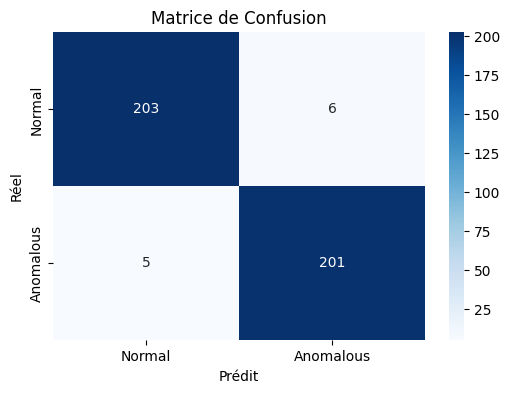
\includegraphics[width=0.49\columnwidth]{confusion_matrix_mlp_service.png}%
    \label{fig:mlp-svc-cm}}%
  \hfill%
  \subfloat[Courbe de perte]{%
    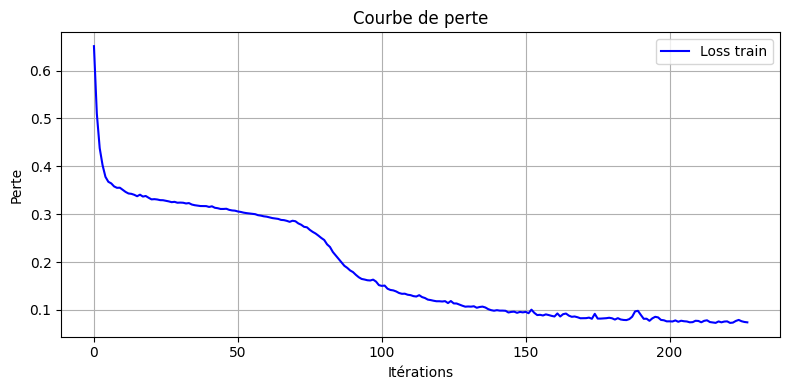
\includegraphics[width=0.49\columnwidth]{loss_curve_mlp_service.png}%
    \label{fig:mlp-svc-loss}}%
  \caption{MLP — \textbf{niveau service}.}
  \label{fig:mlp-service}
\end{figure}

\FloatBarrier
% --------- MLP — NIVEAU APPLICATION (images puis explications) ----------
\paragraph{Niveau application.}

\begin{figure}[!t]
  \centering
  \subfloat[Matrice de confusion]{%
    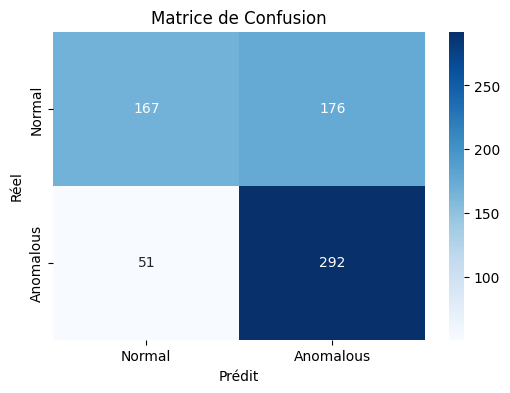
\includegraphics[width=0.49\columnwidth]{confusion_matrix_mlp_application.png}%
    \label{fig:mlp-app-cm}}%
  \hfill%
  \subfloat[Courbe de perte]{%
    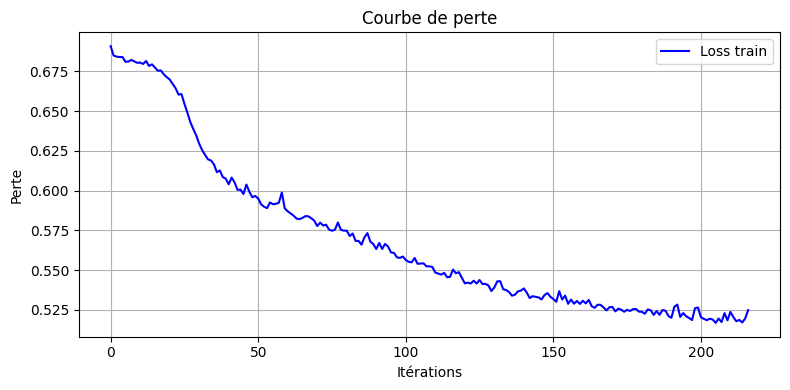
\includegraphics[width=0.49\columnwidth]{loss_curve_mlp_application.png}%
    \label{fig:mlp-app-loss}}%
  \caption{MLP — \textbf{niveau application}.}
  \label{fig:mlp-app}
\end{figure}

\textbf{Résumé des métriques.}
\begin{itemize}
    \item Accuracy = 0{,}52 \quad
          Precision = 0{,}62 \quad
          Recall = 0{,}12 \quad
          F1-score = 0{,}20
\end{itemize}

\textbf{Analyse.}
La matrice (\textit{fig \ref{fig:mlp-app}.\subref{fig:mlp-app-cm}}) révèle un grand nombre de faux négatifs (rappel très faible) : le modèle manque une large partie des anomalies. 
Malgré une perte finale basse (\textit{fig \ref{fig:mlp-app}.\subref{fig:mlp-app-loss}}), la généralisation reste médiocre, suggérant un surapprentissage sur des motifs faiblement discriminants.

\paragraph{Lecture croisée.}
Au \textbf{niveau service}, la granularité fine (latences spécifiques, distribution détaillée des codes HTTP, variabilité locale) fournit des signaux nets que le MLP sépare efficacement. 
Au \textbf{niveau application}, l’agrégation dilue ces signaux et masque les anomalies locales ; le modèle apprend des motifs peu généralisables, expliquant le \textit{recall} très bas malgré une courbe de perte visuellement “propre”.

\subsubsection{\textbf{Autoencodeur LSTM}}

L’autoencodeur LSTM a été conçu pour apprendre uniquement la structure des données normales.  
En phase d’inférence, les observations présentant une erreur de reconstruction supérieure à un seuil prédéfini sont considérées comme des anomalies.  
Cette approche est particulièrement adaptée aux séries temporelles, car les couches LSTM capturent les dépendances temporelles et les dynamiques séquentielles.

% --------- LSTM — NIVEAU SERVICE (images puis explications) ----------
\paragraph{Niveau service.}

\begin{figure}[!t]
  \centering
  \subfloat[Matrice de confusion]{%
    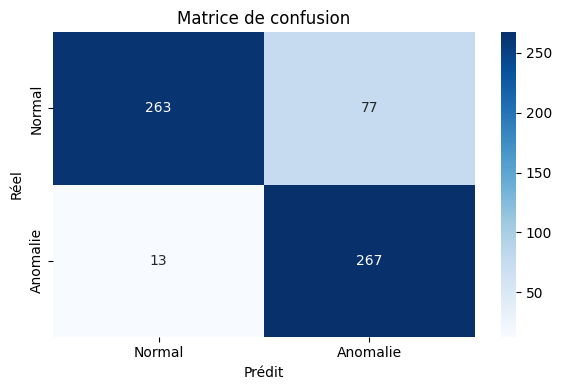
\includegraphics[width=0.49\columnwidth]{confusion_matrix_lstm_service.png}%
    \label{fig:lstm-svc-cm}}%
  \hfill%
  \subfloat[Courbe de perte]{%
    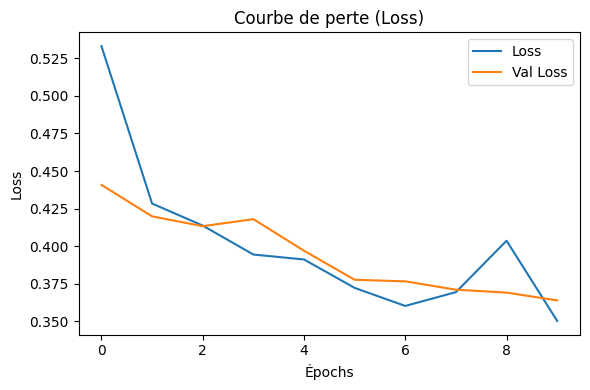
\includegraphics[width=0.49\columnwidth]{loss_curve_lstm_service.png}%
    \label{fig:lstm-svc-loss}}%
  \caption{LSTM autoencodeur — \textbf{niveau service}.}
  \label{fig:lstm-service}
\end{figure}

\textbf{Résumé des métriques.}
\begin{itemize}
    \item Accuracy = 0{,}85 \quad
          Precision = 0{,}78 \quad
          Recall = 0{,}95 \quad
          F1-score = 0{,}86
\end{itemize}

\textbf{Analyse.}
La matrice de confusion (\textit{fig \ref{fig:lstm-service}.\subref{fig:lstm-svc-cm}}) montre que sur 550 échantillons normaux, 263 sont correctement classés et 77 faussement signalés comme anomalies.  
Pour les anomalies, 267 sur 280 sont détectées correctement, expliquant le \textbf{rappel élevé (95\,\%)}.  
Cette sensibilité réduit le risque de laisser passer des anomalies, tandis que la précision de 0{,}78 traduit encore 22\,\% de faux positifs (fluctuations normales interprétées comme anomalies).

\textbf{Courbe de perte.}
La courbe (\textit{fig \ref{fig:lstm-service}.\subref{fig:lstm-svc-loss}}) illustre un apprentissage stable :
\begin{enumerate}
    \item \textbf{Phase initiale (0--2 époques)} : forte baisse (de $\approx 0{,}69$ à $\approx 0{,}67$), capture rapide des structures majeures.
    \item \textbf{Phase intermédiaire (3--6 époques)} : décroissance plus lente, ajustement sur des motifs subtils.
    \item \textbf{Phase finale (7--9 époques)} : perte $\approx 0{,}63$ avec validation parallèle, convergence sans surapprentissage notable.
\end{enumerate}

\textbf{Interprétation.}
Le couple \textit{rappel élevé} / \textit{précision modérée} correspond au compromis classique en détection d’anomalies : on privilégie la sensibilité au prix de davantage de fausses alertes — acceptable en supervision critique.

% --------- LSTM — NIVEAU APPLICATION (images puis explications) ----------
\paragraph{Niveau application.}

\begin{figure}[!t]
  \centering
  \subfloat[Matrice de confusion]{%
    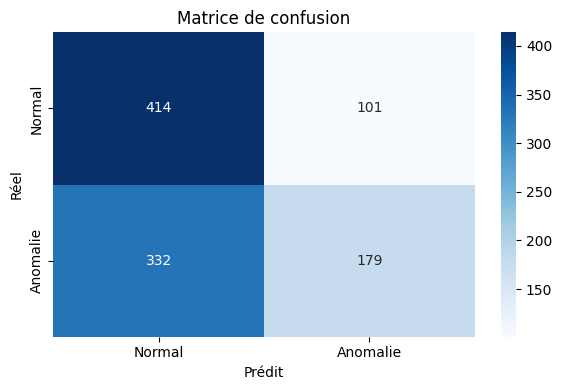
\includegraphics[width=0.49\columnwidth]{confusion_matrix_lstm_application.png}%
    \label{fig:lstm-app-cm}}%
  \hfill%
  \subfloat[Courbe de perte]{%
    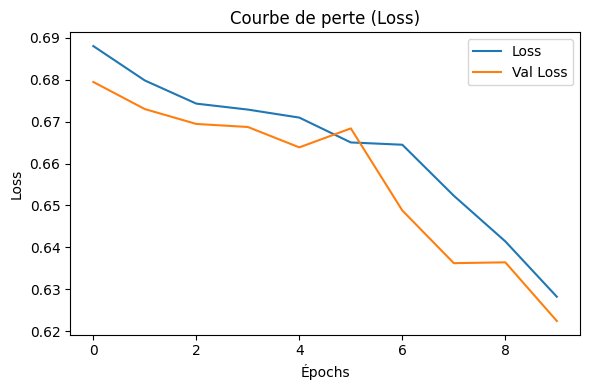
\includegraphics[width=0.49\columnwidth]{loss_curve_lstm_application.png}%
    \label{fig:lstm-app-loss}}%
  \caption{LSTM autoencodeur — \textbf{niveau application}.}
  \label{fig:lstm-app}
\end{figure}

\textbf{Résumé des métriques.}
\begin{itemize}
    \item Accuracy = 0{,}58 \quad
          Precision = 0{,}64 \quad
          Recall = 0{,}35 \quad
          F1-score = 0{,}45
\end{itemize}

\textbf{Analyse.}
La matrice (\textit{fig \ref{fig:lstm-app}.\subref{fig:lstm-app-cm}}) révèle que sur 515 échantillons normaux, 414 sont correctement classés mais 101 sont faussement détectés comme anomalies.  
Sur 511 anomalies réelles, seules 179 sont détectées, laissant 332 faux négatifs — d’où le \textbf{rappel faible (35\,\%)} — signe de la difficulté à distinguer anomalies et fluctuations normales au niveau agrégé.

\textbf{Courbe de perte.}
Le profil (\textit{fig \ref{fig:lstm-app}.\subref{fig:lstm-app-loss}}) diffère du niveau service :
\begin{enumerate}
    \item \textbf{Phase initiale (0--1 époque)} : perte passant de $\approx 0{,}53$ à $\approx 0{,}43$.
    \item \textbf{Phase intermédiaire (2--6 époques)} : poursuite de la baisse avec fluctuations, apprentissage moins stable.
    \item \textbf{Phase finale (7--9 époques)} : convergence vers $\approx 0{,}35$ sans gain de rappel, suggérant un surajustement aux motifs d’entraînement.
\end{enumerate}

\textbf{Interprétation.}
Les signaux applicatifs, plus bruités et moins corrélés temporellement, font perdre à l’autoencodeur LSTM son avantage séquentiel.  
Faute de motifs discriminants nets après agrégation, une proportion importante d’anomalies n’est pas détectée.
\FloatBarrier


\subsubsection{\textbf{Modèle hybride LSTM + MLP}}

Le modèle hybride vise à combiner deux paradigmes complémentaires :
\begin{itemize}
    \item \textbf{LSTM} : exploite les dépendances temporelles pour analyser les variations séquentielles et contextuelles des métriques.
    \item \textbf{MLP} : traite efficacement les variables indépendantes ou faiblement corrélées dans un cadre non séquentiel, permettant d’intégrer des signaux plus statiques.
\end{itemize}
La logique sous-jacente est que les métriques issues d’un environnement microservices contiennent à la fois des patterns dynamiques (latence, throughput) et des informations plus stables (répartition des codes HTTP, moyennes glissantes). En combinant ces deux approches, le modèle cherche à capturer simultanément la dimension temporelle et la dimension statique.

% --------- HYBRIDE — NIVEAU SERVICE (images puis explications) ----------
\paragraph{Niveau service.}

\textbf{Performances globales.}
\begin{itemize}
    \item Accuracy = 0{,}91 \quad
          Precision = 0{,}87 \quad
          Recall = 0{,}97 \quad
          F1-score = 0{,}92
\end{itemize}

\textbf{Analyse.}
La matrice (\textit{fig \ref{fig:hybrid-service}.\subref{fig:hyb-svc-cm}}) montre un \textbf{rappel élevé (97\,\%)} : les anomalies sont détectées presque intégralement.  
Le volume de faux positifs est inférieur à celui du LSTM seul, ce qui suggère que la composante MLP filtre des fluctuations normales.
\FloatBarrier
\begin{figure}[!t]
  \centering
  \subfloat[Matrice de confusion]{%
    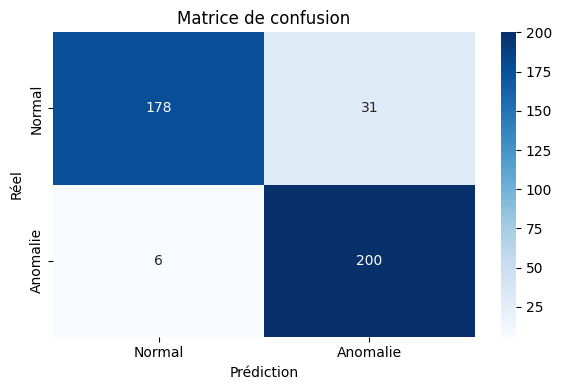
\includegraphics[width=0.49\columnwidth]{confusion_matrix_hybrid_service.png}%
    \label{fig:hyb-svc-cm}}%
  \hfill%
  \subfloat[Courbe d’apprentissage]{%
    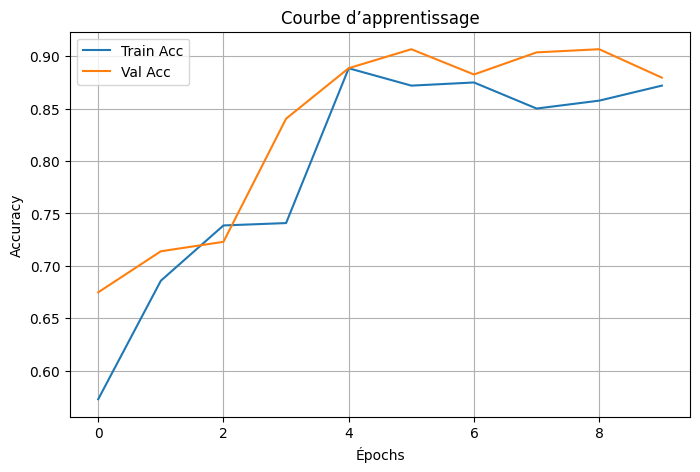
\includegraphics[width=0.49\columnwidth]{loss_curve_hybrid_service.png}%
    \label{fig:hyb-svc-curve}}%
  \caption{Modèle hybride — \textbf{niveau service}.}
  \label{fig:hybrid-service}
\end{figure}

\textbf{Courbe d’apprentissage.}
La courbe (\textit{fig \ref{fig:hybrid-service}.\subref{fig:hyb-svc-curve}}) présente une montée rapide puis une convergence stable, avec peu d’écart entraînement/validation — \emph{surapprentissage limité}.

\textbf{Interprétation.}
Au niveau service, des signaux stables et structurés permettent au LSTM de capter la dynamique, tandis que le MLP stabilise la décision finale. Le compromis \textit{sensibilité/spécificité} est favorable : moins de fausses alertes sans perte des vraies anomalies.

% --------- HYBRIDE — NIVEAU APPLICATION (images puis explications) ----------
\paragraph{Niveau application.}

\begin{figure}[!t]
  \centering
  \subfloat[Matrice de confusion]{%
    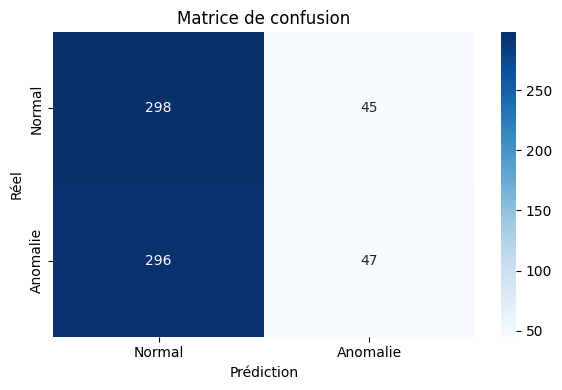
\includegraphics[width=0.49\columnwidth]{confusion_matrix_hybrid_application.png}%
    \label{fig:hyb-app-cm}}%
  \hfill%
  \subfloat[Courbe d’apprentissage]{%
    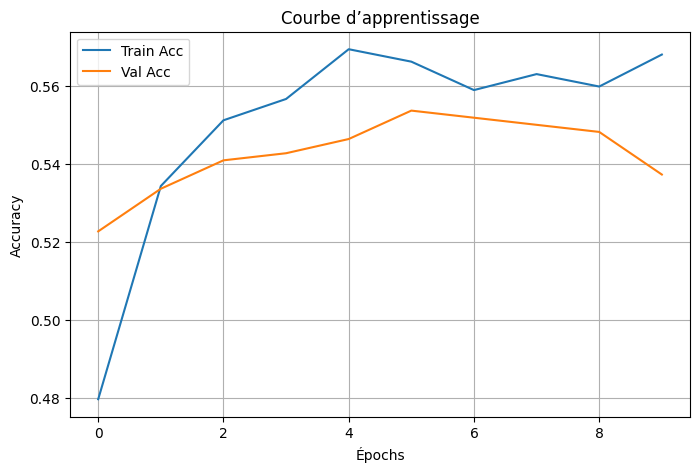
\includegraphics[width=0.49\columnwidth]{loss_curve_hybrid_application.png}%
    \label{fig:hyb-app-curve}}%
  \caption{Modèle hybride — \textbf{niveau application}.}
  \label{fig:hybrid-app}
\end{figure}

\textbf{Performances globales.}
\begin{itemize}
    \item Accuracy = 0{,}50 \quad
          Precision = 0{,}51 \quad
          Recall = 0{,}14 \quad
          F1-score = 0{,}22
\end{itemize}

\textbf{Analyse.}
La matrice (\textit{fig \ref{fig:hybrid-app}.\subref{fig:hyb-app-cm}}) met en évidence une \textbf{chute du rappel (14\,\%)} : la majorité des anomalies échappent à la détection, avec de nombreux faux négatifs.

\textbf{Courbe d’apprentissage.}
La courbe (\textit{fig \ref{fig:hybrid-app}.\subref{fig:hyb-app-curve}}) progresse lentement puis atteint un \emph{plateau prématuré}. La faible marge entraînement/validation indique que la limite vient surtout de la nature des données (signaux dilués) plutôt que d’un manque de capacité du modèle.

\textbf{Interprétation.}
Au niveau application, l’agrégation dilue les signaux temporels et masque les anomalies locales : la composante LSTM perd en pertinence et le MLP, privé de variables distinctives, ne compense pas. Le gain de l’hybride n’apparaît que si les données contiennent des informations discriminantes suffisantes — ce qui est vrai au niveau service, beaucoup moins au niveau application.


\subsubsection{Résumé comparatif et tendances}

\paragraph{Observation générale :}
Trois tendances structurantes se dégagent de l'analyse :
\begin{enumerate}
    \item \textbf{Supériorité systématique des performances au niveau service} :  
    Les trois modèles obtiennent des scores nettement plus élevés lorsqu'ils sont appliqués sur les données désagrégées par service. Cette différence s’explique par la richesse des signaux capturés à ce niveau : latences spécifiques, variations locales de charge, distribution fine des codes HTTP.  
    En revanche, au niveau application, l’agrégation des métriques dilue ces signaux et atténue les ruptures temporelles, ce qui rend la tâche de détection plus complexe. Les modèles doivent alors inférer des anomalies à partir de motifs beaucoup moins distinctifs.

    \item \textbf{Limitation du LSTM par la granularité des données} :  
    Le LSTM excelle dans la modélisation de séries temporelles lorsqu'il existe une structure séquentielle forte. Au niveau service, cette condition est remplie, et le modèle atteint un rappel élevé (95\%), détectant presque toutes les anomalies.  
    Cependant, lorsque les données sont agrégées au niveau application, les patterns temporels deviennent moins marqués, entraînant une chute significative du rappel (35\%). Autrement dit, la valeur ajoutée du LSTM est directement proportionnelle à la clarté des dépendances temporelles dans les données d’entrée.

    \item \textbf{Rendement conditionnel des modèles hybrides} :  
    La combinaison LSTM + MLP offre un compromis solide au niveau service (F1-score = 0.92) grâce à la complémentarité entre :
    \begin{itemize}
        \item le LSTM, qui capture les dynamiques temporelles ;
        \item le MLP, qui filtre les variations normales et améliore la précision.
    \end{itemize}
    En revanche, au niveau application, cette combinaison ne parvient pas à compenser le manque de signaux discriminants. Les performances restent proches, voire inférieures, à celles des modèles individuels. Cela illustre un principe clé : un modèle complexe ne surperforme que si les données contiennent des informations distinctives exploitables.
\end{enumerate}

\paragraph{Lecture stratégique des résultats :}
\begin{itemize}
    \item Pour un déploiement opérationnel où la granularité des métriques est fine (niveau service), le \textbf{MLP} reste la solution la plus efficace en précision globale, tandis que le \textbf{LSTM} et l’hybride sont préférés si la sensibilité aux anomalies (rappel élevé) est prioritaire.
    \item Dans des contextes où seules des métriques agrégées au niveau application sont disponibles, les performances sont limitées quelle que soit l’architecture utilisée. L’enjeu devient alors moins un choix de modèle qu’une optimisation de la collecte de données pour augmenter la qualité du signal.
    \item Ces résultats rappellent l’importance de l’alignement entre la nature des données et la conception du modèle : la sophistication algorithmique n’apporte un gain que si elle répond à une structure exploitable dans les données.
\end{itemize}

\begin{table}[!t]
\centering
\caption{Résumé comparatif des performances des modèles sur les deux niveaux d'analyse.}
\label{tab:resume-perf}
\begin{tabular}{@{}l l c c c c@{}}
\toprule
\textbf{Modèle} & \textbf{Niveau} & \textbf{Acc.} & \textbf{Prec.} & \textbf{Rec.} & \textbf{F1} \\
\midrule
MLP & Service & 0.97 & 0.97 & 0.98 & 0.97 \\
MLP & Application & 0.52 & 0.62 & 0.12 & 0.20 \\
LSTM & Service & 0.85 & 0.78 & 0.95 & 0.86 \\
LSTM & Application & 0.58 & 0.64 & 0.35 & 0.45 \\
Hybride & Service & 0.91 & 0.87 & 0.97 & 0.92 \\
Hybride & Application & 0.50 & 0.51 & 0.14 & 0.22 \\
\bottomrule
\end{tabular}
\end{table}


\subsection{Discussion}

Les résultats confirment un écart net entre \textbf{niveau service} et \textbf{niveau application}. Ce contraste s’explique d’abord par la granularité des signaux, avec des conséquences directes sur la détectabilité des anomalies et l’utilité relative des architectures.

\subsubsection*{Analyse par niveau}

\paragraph{Au niveau service.}
Signaux temporels et statistiques \emph{clairs} (latences, répartitions HTTP, variations locales) et variabilité modérée $\Rightarrow$ modèles facilités.
\begin{itemize}
  \item \textbf{MLP} : sépare efficacement des relations non linéaires sans dépendances séquentielles complexes.
  \item \textbf{LSTM} : capte les motifs séquentiels, \textit{rappel} très élevé (détection quasi exhaustive).
  \item \textbf{Hybride} : combine sensibilité (LSTM) et stabilité décisionnelle (MLP), moins de faux positifs.
\end{itemize}
\emph{Conclusion} : des signaux forts et localisés expliquent des \textit{accuracy} souvent $>90\%$.

\paragraph{Au niveau application.}
Agrégation multi‐services $\Rightarrow$ dilution des signaux et bruit statistique ; une dégradation locale peut être masquée par le reste.
\begin{itemize}
  \item \textbf{MLP} : frontières de décision floues, \textit{rappel} très faible (p.\,ex. $12\%$).
  \item \textbf{LSTM} : quelques motifs globaux captés, mais \textit{rappel} modeste faute de structure temporelle marquée.
  \item \textbf{Hybride} : peu d’apport, la limite vient surtout de l’information disponible, pas du choix d’architecture.
\end{itemize}
\emph{Conclusion} : la granularité des données conditionne la sensibilité ; l’agrégation excessive la réduit fortement.

\subsubsection*{Forces et limites des approches}

\begin{itemize}
  \item \textbf{MLP} — \emph{Forces} : simple, rapide, robuste avec signaux statiques/forts. \emph{Limites} : ne capture pas les dynamiques séquentielles, sensible au bruit agrégé.
  \item \textbf{Autoencodeur LSTM} — \emph{Forces} : excellente sensibilité aux anomalies subtiles (modélisation séquentielle), utile quand les FN coûtent cher. \emph{Limites} : seuil d’erreur crucial, davantage de FP, entraînement plus coûteux.
  \item \textbf{Hybride LSTM+MLP} — \emph{Forces} : couvre variables temporelles et statiques, bon compromis quand les signaux sont variés. \emph{Limites} : complexité accrue sans gain si l’information discriminante est faible.
\end{itemize}

\subsubsection*{Implications pratiques}

\begin{itemize}
  \item Privilégier la \textbf{surveillance au niveau service} pour des détections rapides et localisées.
  \item Conserver une \textbf{vue application} pour les tendances globales et pannes étendues, en acceptant une sensibilité moindre.
  \item \textbf{Combiner les deux niveaux} en production (collecte fine + agrégée) pour maximiser couverture et réactivité.
\end{itemize}



\section{Conclusion and Future Work}

Ce travail a exploré et comparé trois approches d'apprentissage automatique pour la détection d'anomalies dans des environnements microservices : un perceptron multicouche (MLP), un autoencodeur LSTM et un modèle hybride LSTM+MLP. Les expérimentations, menées aux niveaux \textit{service} et \textit{application} et évaluées via l’accuracy, la précision, le rappel et le F1-score, ont permis de dégager plusieurs constats.

Les résultats montrent une nette supériorité du suivi au niveau \textit{service}, avec un F1-score atteignant 0.97 pour le MLP, alors que les performances chutent fortement au niveau \textit{application} en raison de la perte de granularité et de la dilution des signaux. Les modèles plus complexes, tels que le LSTM ou l’hybride, n’apportent un gain significatif que lorsque des motifs temporels marqués coexistent avec des variables statiques informatives.

Ces observations soulignent que la granularité et la qualité des données influencent davantage les performances que la seule complexité algorithmique, et que le choix du modèle doit être aligné avec la nature des signaux surveillés.

Les perspectives de ce travail incluent : (i) l’enrichissement des données avec des journaux applicatifs, des traces distribuées et des métriques métier ; (ii) l’exploration d’architectures intégrant des mécanismes d’attention pour mieux capter les dépendances à long terme ; (iii) l’intégration de méthodes d’explicabilité telles que SHAP ou LIME afin d’améliorer la transparence et l’adoption par les équipes DevOps ; et (iv) la validation de ces approches en environnement de production.

Ces résultats ouvrent la voie à des systèmes de détection d’anomalies plus précis, interprétables et adaptés aux contraintes opérationnelles des architectures microservices modernes.


\nocite{*}
\bibliographystyle{IEEEtran}
\bibliography{references}

\end{document}
